\documentclass[tikz,border=4pt]{standalone}
\usepackage{ctex}
\usepackage{pgfplots}
\pgfplotsset{compat=1.18}
\begin{document}
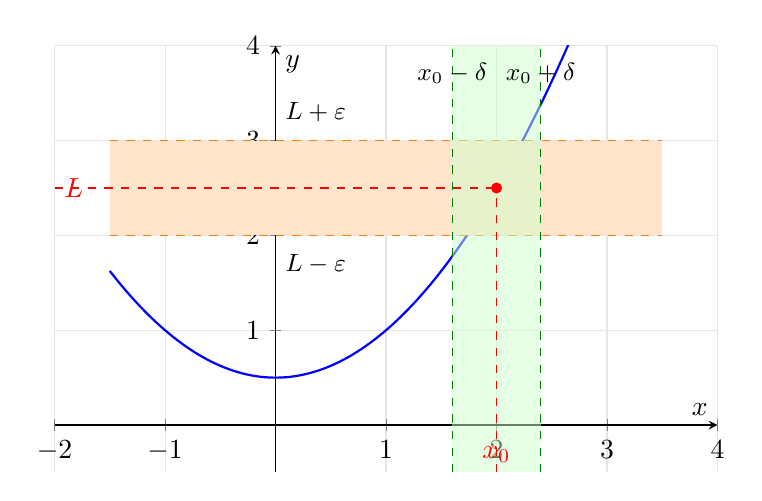
\begin{tikzpicture}
\begin{axis}[
    axis lines=middle, width=10cm, height=7cm,
    xmin=-2, xmax=4, ymin=-0.5, ymax=4,
    xlabel={$x$}, ylabel={$y$},
    grid=both, grid style={gray!20},
    samples=200,
]
% 函数 f(x) = 0.5x^2 + 0.5, 在 x_0=2 处 L=2.5
\addplot[blue, thick, domain=-1.5:3.5] {0.5*x^2 + 0.5};
% ε 带
\fill[orange!20] (axis cs:-1.5,2.0) rectangle (axis cs:3.5,3.0);
\draw[dashed, orange] (axis cs:-1.5,2.0) -- (axis cs:3.5,2.0);
\draw[dashed, orange] (axis cs:-1.5,3.0) -- (axis cs:3.5,3.0);
% δ 带
\fill[green!20, opacity=0.5] (axis cs:1.6,-0.5) rectangle (axis cs:2.4,4);
\draw[dashed, green!50!black] (axis cs:1.6,-0.5) -- (axis cs:1.6,4);
\draw[dashed, green!50!black] (axis cs:2.4,-0.5) -- (axis cs:2.4,4);
% L 和 x_0
\draw[red, dashed] (axis cs:2,-0.5) -- (axis cs:2,2.5);
\draw[red, dashed] (axis cs:-2,2.5) -- (axis cs:2,2.5);
\node[red, anchor=west] at (axis cs:-2, 2.5) {$L$};
\node[red, anchor=south] at (axis cs:2, -0.5) {$x_0$};
\node[anchor=west] at (axis cs:0, 3.3) {\small $L+\varepsilon$};
\node[anchor=west] at (axis cs:0, 1.7) {\small $L-\varepsilon$};
\node[anchor=south] at (axis cs:1.6, 3.5) {\small $x_0-\delta$};
\node[anchor=south] at (axis cs:2.4, 3.5) {\small $x_0+\delta$};
\fill[red] (axis cs:2,2.5) circle (2pt);
\end{axis}
\end{tikzpicture}
\end{document}
